\documentclass[10pt, a4paper]{article}
\usepackage{lrec}
%\usepackage{multibib}
%\newcites{languageresource}{Language Resources}
\usepackage{graphicx}
\usepackage{tabularx}
\usepackage{soul}
% for eps graphics

\usepackage{epstopdf}
\usepackage[latin1]{inputenc}

\usepackage{hyperref}
\usepackage{xstring}

\newcommand{\secref}[1]{\StrSubstitute{\getrefnumber{#1}}{.}{ }}

\title{Title of the LREC 2020 Paper (Title in 14-point Times New Roman Bold)\\ \vspace*{.5\baselineskip} \normalfont{ The Title \ul{Must Be} Capitalised as in:\\ \vspace*{.5\baselineskip} \textbf{The Rise and Fall of Ziggy Stardust and the Spiders from Mars}}}

\name{Author1, Author2, Author3}

\address{Affiliation1, Affiliation2, Affiliation3 \\
         Address1, Address2, Address3 \\
         author1@xxx.yy, author2@zzz.edu, author3@hhh.com\\
         \{author1, author5, author9\}@abc.org\\}


\abstract{
Each article (full paper) must include an abstract of 150 to 200 words in Times New Roman
9 with interlinear spacing of 10 pt. The heading Abstract should be
centred, font Times New Roman 10 bold. This short abstract will also be used
for producing the Booklet of Abstracts (PDF) containing the abstracts of all
papers presented at the Conference. \\ \newline \Keywords{keyword1, keyword2,
keyword3} }

\begin{document}

\maketitleabstract

\section{Full Paper and not an Extended Abstract}

LREC2020 is moving to full paper submissions. Each submitted paper should be submitted on white A4 paper. The fully
justified text should be formatted in two parallel columns, each 8.25 cm wide,
and separated by a space of 0.63 cm. Left, right, and bottom margins should be
1.9 cm and the top margin 2.5 cm. The font for the main body of the text should
be Times New Roman 10 with interlinear spacing of 11 pt.

\subsection{General Instructions for the Submitted Full Paper}

Each submitted paper  should be between \ul{a minimum of four  and
a maximum of eight  pages including figures}.

\section{Full Paper}

Each manuscript should be submitted on white A4 paper. The fully
justified text should be formatted in two parallel columns, each 8.25 cm wide,
and separated by a space of 0.63 cm. Left, right, and bottom margins should be
1.9 cm. and the top margin 2.5 cm. The font for the main body of the text should
be Times New Roman 10 with interlinear spacing of 12 pt.  Articles must be
between 4 and 8 pages in length, regardless of the mode of presentation (oral
or poster).

\subsection{General Instructions for the Final Paper}

Each paper is allocated between \ul{a minimum of four and a maximum of
eight pages including figures}. The unprotected PDF files will appear in the
on-line proceedings directly as received. Do not print the page number.

\section{Page Numbering}

\textbf{Please do not include page numbers in your article.} The definitive page
numbering of articles published in the proceedings will be decided by the
organising committee.

\section{Headings / Level 1 Headings}

Headings should be capitalised in the same way as the main title, and centred
within the column. The font used is Times New Roman 12 bold. There should
also be a space of 12 pt between the title and the preceding section, and
a space of 3 pt between the title and the text following it.

\subsection{Level 2 Headings}

The format for level 2 headings is the same as for level 1 Headings, with the
font Times New Roman 11, and the heading is justified to the left of the column.
There should also be a space of 6 pt between the title and the preceding
section, and a space of 3 pt between the title and the text following it.

\subsubsection{Level 3 Headings}

The format for level 3 headings is the same as for level 2 headings, except that
the font is Times New Roman 10, and there should be no space left between the
heading and the text. There should also be a space of 6 pt between the title and
the preceding section, and a space of 3 pt between the title and the text
following it.

%\subsubsection{Example of a sub-subsection with a long heading that will occupy two lines}
%
%Yet another example of a sub-subsection. Yet another example of a sub-subsection. Yet another example of a sub-subsection. Yet another example of a sub-subsection. Yet another example of a sub-subsection.

\section{Citing References in the Text}

\subsection{Bibliographical References}

All bibliographical references within the text should be put in between
parentheses with the author's surname followed by a comma before the date
of publication,\cite{Martin-90}. If the sentence already includes the author's
name, then it is only necessary to put the date in parentheses:
\newcite{Martin-90}. When several authors are cited, those references should be
separated with a semicolon: \cite{Martin-90,CastorPollux-92}. When the reference
has more than three authors, only cite the name of the first author followed by
``et al.'' (e.g. \cite{Superman-Batman-Catwoman-Spiderman-00}).

\subsection{Language Resource References}

\subsubsection{When Citing Language Resources}

When citing language resources, we recommend to proceed in the same way to
bibliographical references.
Thus, a language resource should be cited as \cite{speecon}.


\section{Figures \& Tables}
\subsection{Figures}

All figures should be centred and clearly distinguishable. They should never be
drawn by hand, and the lines must be very dark in order to ensure a high-quality
printed version. Figures should be numbered in the text, and have a caption in
Times New Roman 10 pt underneath. A space must be left between each figure and
its respective caption. 

Example of a figure enclosed in a box:

\begin{figure}[!h]
\begin{center}
%\fbox{\parbox{6cm}{
%This is a figure with a caption.}}
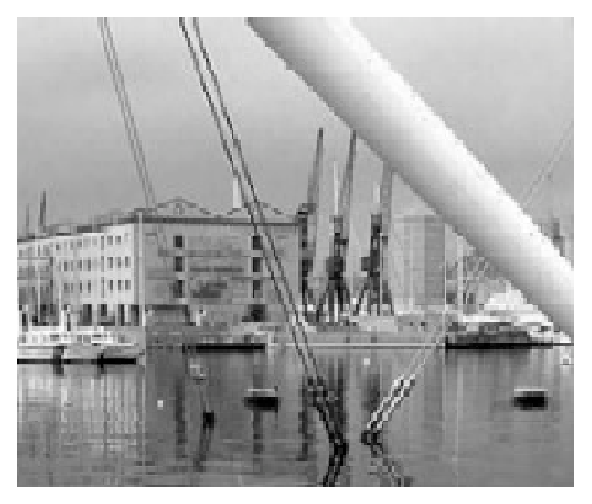
\includegraphics[scale=0.5]{lrec2020W-image1.eps} 
\caption{The caption of the figure.}
\label{fig.1}
\end{center}
\end{figure}

Figure and caption should always appear together on the same page. Large figures
can be centred, using a full page.
%NB: an example of large figures is missing.  \newpage

\subsection{Tables}

The instructions for tables are the same as for figures.
%Two types of tables are distinguished: in-column and big tables that don't fit in the columns.
%\subsection{In-column tables}
%An example of an in-column table is presented here.
%
\begin{table}[!h]
\begin{center}
\begin{tabularx}{\columnwidth}{|l|X|}

      \hline
      Level&Tools\\
      \hline
      Morphology & Pitrat Analyser\\
      \hline
      Syntax & LFG Analyser (C-Structure)\\
      \hline
     Semantics & LFG F-Structures + Sowa's\\
     & Conceptual Graphs\\
      \hline

\end{tabularx}
\caption{The caption of the table}
 \end{center}
\end{table}

%\subsection{Big tables}
%
%An example of a big table which extends beyond the column and will
%float in the next page.
%
% \begin{table*}[ht]
% \begin{center}
% \begin{tabular}{|l|l|}
%
%       \hline
%       Level&Tools\\
%       \hline\hline
%       Morphology & Pitrat Analyser\\
%       Syntax & LFG Analyser (C-Structure)\\
%       Semantics & LFG F-Structures + Sowa's Conceptual Graphs  \\
%       \hline
%
% \end{tabular}
% \caption{The caption of the big table}
% \end{center}
% \end{table*}
%

\section{Footnotes}

Footnotes are indicated within the text by a number in
superscript\footnote{Footnotes should be in Times New Roman 9 pt, and appear at
the bottom of the same page as their corresponding number. Footnotes should also
be separated from the rest of the text by a horizontal line 5 cm long.}.

\section{Copyrights}

The Language Resouces and Evaluation Conference (LREC)
proceedings are published by the European Language Resources Association (ELRA).
They are available online from the conference website.


ELRA's policy is to acquire copyright for all LREC contributions. In assigning
your copyright, you are not forfeiting your right to use your contribution
elsewhere. This you may do without seeking permission and is subject only to
normal acknowledgement to the LREC proceedings. The LREC 2020 Proceedings are
licensed under CC-BY-NC, the Creative Commons Attribution-Non-Commercial 4.0
International License.

\section{Conclusion}

Your submission of a finalised contribution for inclusion in the LREC
proceedings automatically assigns the above-mentioned copyright to ELRA.


\section{Acknowledgements}

Place all acknowledgements (including those concerning research grants and
funding) in a separate section at the end of the article.

\section{Providing References}

\subsection{Bibliographical References}
Bibliographical references should be listed in alphabetical order at the
end of the article. The title of the section, ``Bibliographical References'',
should be a level 1 heading. The first line of each bibliographical reference
should be justified to the left of the column, and the rest of the entry should
be indented by 0.35 cm.

The examples provided in Section \secref{main:ref} (some of which are fictitious
references) illustrate the basic format required for articles in conference
proceedings, books, journal articles, PhD theses, and chapters of books.

\subsection{Language Resource References}

Language resource references should be listed in alphabetical order at the end
of the article.

\section*{Appendix: How to Produce the \texttt{.pdf} Version}

In order to generate a PDF file out of the LaTeX file herein, when citing
language resources, the following steps need to be performed:

\begin{itemize}
    \item{Compile the \texttt{.tex} file once}
    \item{Invoke \texttt{bibtex} on the eponymous \texttt{.aux} file}
 %   \item{Invoke \texttt{bibtex} on the \texttt{languageresources.aux} file}
    \item{Compile the \texttt{.tex} file twice}
\end{itemize}

% \nocite{*}
\section{Bibliographical References}
\label{main:ref}

\bibliographystyle{lrec}
\bibliography{lrec2020W-xample}


%\section{Language Resource References}
%\label{lr:ref}
%\bibliographystylelanguageresource{lrec}
%\bibliographylanguageresource{lrec2020W-xample}

\end{document}
